%-------------------------
% Resume in LaTeX
% Author : Miguel Peixoto
% Based on template by : Sourabh Bajaj
% License : MIT
%------------------------

\documentclass[letterpaper,11pt]{article}

\usepackage{latexsym}
\usepackage[empty]{fullpage}
\usepackage{titlesec}
\usepackage{marvosym}
\usepackage[usenames,dvipsnames]{color}
\usepackage{verbatim}
\usepackage{enumitem}
\usepackage[hidelinks]{hyperref}
\usepackage{fancyhdr}
\usepackage[english]{babel}
\usepackage{tabularx}
\usepackage{graphicx}
\usepackage{tikz}
\usepackage[table]{xcolor}
\input{glyphtounicode}

\pagestyle{fancy}
\fancyhf{} % Clear all header and footer fields
\fancyfoot{}
\renewcommand{\headrulewidth}{0pt}
\renewcommand{\footrulewidth}{0pt}

% Adjust margins
\addtolength{\oddsidemargin}{-0.5in}
\addtolength{\evensidemargin}{-0.5in}
\addtolength{\textwidth}{1in}
\addtolength{\topmargin}{-.5in}
\addtolength{\textheight}{1.0in}

\urlstyle{same}

\raggedbottom
\raggedright
\setlength{\tabcolsep}{0in}

% Sections formatting
\titleformat{\section}{
  \vspace{-4pt}\scshape\raggedright\large
}{}{0em}{}[\color{black}\titlerule \vspace{-5pt}]

% Ensure that generate PDF is machine readable/ATS parsable
\pdfgentounicode=1

%-------------------------
% Custom commands
\newcommand{\resumeItem}[2]{
  \item\small{
    \textbf{#1}{: #2 \vspace{-2pt}}
  }
}

% Just in case someone needs a heading that does not need to be in a list
\newcommand{\resumeHeading}[4]{
    \begin{tabular*}{0.99\textwidth}[t]{l@{\extracolsep{\fill}}r}
      \textbf{#1} & #2 \\
      \textit{\small#3} & \textit{\small #4} \\
    \end{tabular*}\vspace{-5pt}
}

\newcommand{\resumeSubheading}[4]{
  \vspace{-1pt}\item
    \begin{tabular*}{0.97\textwidth}[t]{l@{\extracolsep{\fill}}r}
      \textbf{#1} & #2 \\
      \textit{\small#3} & \textit{\small #4} \\
    \end{tabular*}\vspace{-5pt}
}

\newcommand{\resumeSubSubheading}[2]{
    \begin{tabular*}{0.97\textwidth}{l@{\extracolsep{\fill}}r}
      \textit{\small#1} & \textit{\small #2} \\
    \end{tabular*}\vspace{-5pt}
}

\newcommand{\resumeSubItem}[2]{\resumeItem{#1}{#2}\vspace{-4pt}}

\renewcommand{\labelitemii}{$\circ$}

\newcommand{\resumeSubHeadingListStart}{\begin{itemize}[leftmargin=*]}
\newcommand{\resumeSubHeadingListEnd}{\end{itemize}}
\newcommand{\resumeItemListStart}{\begin{itemize}}
\newcommand{\resumeItemListEnd}{\end{itemize}\vspace{-5pt}}

%-------------------------------------------
%%%%%%  CV STARTS HERE  %%%%%%%%%%%%%%%%%%%%%%%%%%%%

\begin{document}

%----------HEADING-----------------
\vspace*{0pt}
\vspace*{-\topmargin}
\vspace*{-\headheight}
\vspace*{-\headsep}
\vspace*{-1in}
\vspace*{-\baselineskip}
\noindent\hspace*{-\oddsidemargin}\hspace*{-1in}%
\colorbox{gray!10}{%
\makebox[\paperwidth][c]{%
\begin{minipage}{\paperwidth}
\vspace{15pt}
\begin{center}
\begin{tabular*}{0.85\paperwidth}{l@{\hspace{1cm}}l}
  \begin{minipage}[c]{0.12\textwidth}
    \raggedleft
    \begin{tikzpicture}
      \clip (0,0) circle (1.4cm);
      \node[anchor=center] at (0,0) {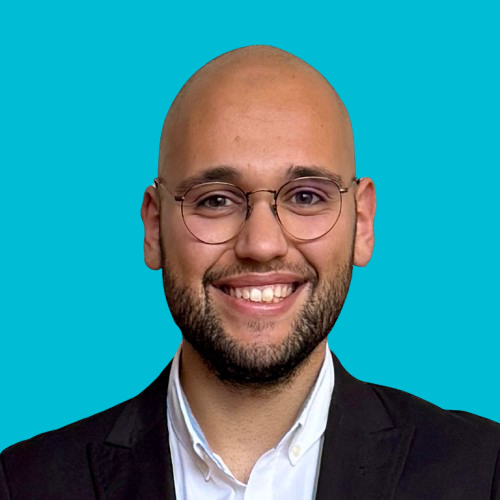
\includegraphics[width=2.8cm,height=2.8cm,keepaspectratio]{photo.png}};
    \end{tikzpicture}
  \end{minipage}
  &
  \begin{minipage}[c]{0.7\textwidth}
    \raggedright
    \textbf{\href{https://miguelpeixoto.net/}{\Large Miguel Peixoto}} \\
    \href{https://miguelpeixoto.net/}{miguelpeixoto.net} \\
    Email: \href{mailto:miguelpeixoto457@gmail.com}{miguelpeixoto457@gmail.com} \\
    GitHub: \href{https://github.com/mcpeixoto}{github.com/mcpeixoto} \\
    Portugal
  \end{minipage}
\end{tabular*}
\end{center}
\vspace{0.5pt}
\end{minipage}%
}%
}

\vspace{1pt}

%-----------EXPERIENCE-----------------
\section{Experience}
  \resumeSubHeadingListStart
    \resumeSubheading
      {Keenfinity (Bosch Spin-off)}{Portugal}
      {AI Architect}{Feb 2025 -- Present}
      \resumeItemListStart
        \resumeItem{Leadership}
          {Leading team of data, frontend and backend engineers across 16 projects in 7 departments.}
        \resumeItem{Projects}
          {Training LLMs from scratch, deploying GenAI frontends/backends, autoencoders for anomaly detection, PDF information extraction/classification/clustering, automatic ticketing with Agentic LLMs, Computer Vision for factory traceability.}
      \resumeItemListEnd

    \resumeSubheading
      {Bosch Security Systems}{Portugal/Germany}
      {Boost Program - Machine Learning Engineer}{Aug 2023 -- Feb 2025}
      \resumeItemListStart
        \resumeItem{Selection}
          {Selected as 1 of 8 from 900+ applicants for Portuguese Junior Managers Program. Mentored by Sergio Salústio, Director of R\&D at Bosch Ovar.}
        \resumeItem{Computer Vision}
          {Developed object detection system for factory material tracking, reducing inefficiencies and scaling to 3 factories worldwide.}
        \resumeItem{Embedded ML}
          {Full ML lifecycle on embedded devices: data engineering, training, fine-tuning, quantization, pruning, compilation and firmware deployment.}
        \resumeItem{AI Solutions}
          {Engaged stakeholders to identify use cases and deploy AI solutions while ensuring compliance and data governance.}
      \resumeItemListEnd

    \resumeSubheading
      {University of Minho}{Braga, Portugal}
      {Researcher}{May 2023 -- Dec 2024}
      \resumeItemListStart
        \resumeItem{Industry Collaboration}
          {Collaborated with Bosch Car Multimedia to advance anomaly detection in industrial applications.}
      \resumeItemListEnd

    \resumeSubheading
      {Instrumentation and Experimental Particle Physics Laboratory}{Braga, Portugal}
      {Researcher}{Oct 2021 -- Present}
      \resumeItemListStart
        \resumeItem{Team Leadership}
          {Led team of 10 students specializing in anomaly detection and quantum computing for high-energy physics.}
        \resumeItem{NLP \& Healthcare}
          {Collaborated with SPAC Lab on disease diagnosis model using Portuguese National Health Service records. Implemented HuggingFace Sentence-Transformers and Facebook Faiss for similarity search.}
        \resumeItem{Quantum ML}
          {Compared Quantum ML architectures with classical methods. Developed robust library with parallelization, unit tests, CI/CD pipelines using Pennylane, Qiskit, PyTorch, and Optuna.}
        \resumeItem{Education}
          {Facilitated machine learning workshops and seminars for research institute students.}
      \resumeItemListEnd

    \resumeSubheading
      {Instrumentation and Experimental Particle Physics Laboratory}{Braga, Portugal}
      {Summer Intern}{Apr 2020 -- Oct 2021}
      \resumeItemListStart
        \resumeItem{Research Projects}
          {Advanced data analysis for dark matter research (2020) and Anomaly Detection for New Physics Discovery at CERN's Large Hadron Collider (2021).}
      \resumeItemListEnd
  \resumeSubHeadingListEnd

%-----------EDUCATION-----------------
\section{Education}
  \resumeSubHeadingListStart
    \resumeSubheading
      {University of Minho}{Braga, Portugal}
      {Master's Degree in Information Physics; Grade: 20/20}{}
      \resumeItemListStart
        \resumeItem{Thesis}
          {Anomaly Detection as a Quality Control Tool in an Industrial Context. Supervised by Prof. Nuno Castro, Director of LIP and National Center for Advanced Computing. Created production-ready autoencoder framework validated at Bosch Braga, outperformed SOTA on MvTec benchmark.}
        \resumeItem{Role}{Student representative of master's program}
      \resumeItemListEnd
    \resumeSubheading
      {University of Minho}{Braga, Portugal}
      {Bachelor's Degree in Physics Engineering; Average Score: 16.4/20}{}
      \resumeItemListStart
        \resumeItem{Leadership}
          {Founded NEFUM Discord community (200+ members), organized national physics students meeting (134 attendees), ran for association president.}
        \resumeItem{Skills Development}{Active member of Academic Debate Association, developing communication and analytical skills.}
      \resumeItemListEnd
  \resumeSubHeadingListEnd

%-----------PUBLICATIONS-----------------
\section{Publications}
  \resumeSubHeadingListStart
    \resumeSubItem{Fitting a Collider in a Quantum Computer}
      {Tackling the Challenges of Quantum Machine Learning for Big Datasets. Frontiers in Artificial Intelligence, 2022. DOI: 10.3389/frai.2023.1268852}
  \resumeSubHeadingListEnd

%-----------AWARDS & HONORS-----------------
\section{Awards \& Honors}
  \resumeSubHeadingListStart
    \resumeSubItem{15th Fraunhofer Portugal Challenge}
      {Recognized for outstanding innovation in technological research for master's thesis.}
    \resumeSubItem{UMinho University Award}
      {Initiation in Scientific Research award for Variational AutoEncoders anomaly detection system in high-energy physics.}
    \resumeSubItem{Empreende@Villa.Jovem-BILATECH}
      {1st place and 5k prize among 30+ finalists for innovative business idea in marketing automation.}
    \resumeSubItem{Meritorious Behavior Award}
      {4 distinctions from Secondary School for participation in "Project Rocket" and Nobel Prize physics seminar.}
  \resumeSubHeadingListEnd

%-----------ADDITIONAL ACTIVITIES-----------------
\section{Additional Activities}
  \resumeSubHeadingListStart
    \resumeSubheading
      {European Researchers' Night - LIP Presentation}{Braga, Portugal}
      {Science Outreach Presenter}{2022}
      \resumeItemListStart
        \resumeItem{Public Engagement}
          {Presented cutting-edge physics research to general public, promoting scientific literacy and inspiring next generation of researchers.}
      \resumeItemListEnd

    \resumeSubheading
      {iQuHACK MIT Hackathon}{Cambridge, MA, USA}
      {Quantum Computing Participant}{2022}
      \resumeItemListStart
        \resumeItem{IonQ Challenge}
          {Competed in prestigious MIT quantum computing hackathon, developing innovative solutions using IonQ's quantum hardware and advancing quantum algorithm development skills.}
      \resumeItemListEnd

    \resumeSubheading
      {ESA Winter Astronomy Camp}{Saint-Barthélemy, Italy}
      {Selected Participant}{2019}
      \resumeItemListStart
        \resumeItem{International Selection}
          {Selected as 1 of 40 participants from 500+ worldwide applications for intensive 1-week astronomy program focused on exoplanet research.}
        \resumeItem{Technical Skills}
          {Engaged in advanced lectures, hands-on observatory activities, and nighttime observations using professional astronomical instruments.}
      \resumeItemListEnd
  \resumeSubHeadingListEnd

%-----------TECHNICAL SKILLS-----------------
\section{Technical Skills}
  \resumeSubHeadingListStart
    \item{
      \textbf{Languages}{: Python, SQL, C++, JavaScript}
      \hfill
      \textbf{ML/AI}{: PyTorch, Scikit-Learn, HuggingFace, TensorFlow}
    }
    \item{
      \textbf{Quantum Computing}{: Pennylane, Qiskit}
      \hfill
      \textbf{Cloud \& Tools}{: Docker, CI/CD, Git, AWS}
    }
    \item{
      \textbf{Computer Vision}{: Object Detection, Anomaly Detection}
      \hfill
      \textbf{NLP}{: Sentence-Transformers, LLMs, GenAI}
    }
  \resumeSubHeadingListEnd

\end{document}
